\documentclass[a4paper,10pt,twoside]{scrartcl}
% \usepackage[pdflatex, tightpage]{preview}
\usepackage[svgnames]{xcolor}
\usepackage{pdflscape}
\usepackage{amsmath,amsfonts}
% \usepackage{graphicx}
\usepackage[left=2cm, right=2cm, top=1.8cm]{geometry}
\usepackage{rotating}
\usepackage{fancyhdr}
\usepackage[texcoord]{eso-pic}
\usepackage[algosection]{algorithm2e}
\usepackage{enumitem}
\usepackage[pdftitle={Repeat Detecter},pdfauthor={Thierry Schuepbach},pdfsubject={PfTools development},baseurl={www.isb-sib.ch}]{hyperref}

\usepackage{tikz, xifthen}
\usetikzlibrary{decorations.markings}
\usetikzlibrary{shapes.geometric}
\usetikzlibrary{positioning,fit}
\usetikzlibrary{calc}

\usepackage[framemethod=default]{mdframed}
\usepackage{enumerate}
\global\mdfdefinestyle{exampledefault}{%
linecolor=lightgray,linewidth=1pt,%
leftmargin=1cm,rightmargin=1cm,
}
\setlist{nolistsep}

\newenvironment{notes}{%
\vspace{0.5em}
\mdfsetup{%
frametitle={\tikz\node[fill=white,rectangle,inner sep=0pt,outer sep=0pt]{Notes};},
frametitleaboveskip=-0.5\ht\strutbox,
frametitlealignment=\raggedright
}%
\begin{mdframed}[style=exampledefault]}{\end{mdframed}}

\pgfdeclarelayer{edgelayer}
\pgfdeclarelayer{nodelayer}
\pgfsetlayers{edgelayer,nodelayer,main}

\tikzstyle{none}=[inner sep=0pt]
\tikzstyle{rn}=[circle,fill=Red,draw=Black,line width=0.8 pt]
\tikzstyle{gn}=[circle,fill=Lime,draw=Black,line width=0.8 pt]
\tikzstyle{yn}=[circle,fill=Yellow,draw=Black,line width=0.8 pt]
\tikzstyle{newstyle}=[circle,fill=White,draw=Black,minimum width=3pt,inner sep=0pt]

\tikzstyle{simple}=[-,draw=Black,line width=2.000]
\tikzstyle{arrow}=[-,draw=Black,postaction={decorate},decoration={markings,mark=at position .5 with {\arrow{>}}},line width=2.000]
\tikzstyle{tick}=[-,draw=Black,postaction={decorate},decoration={markings,mark=at position .5 with {\draw (0,-0.1) -- (0,0.1);}},line width=2.000]

\newcommand*{\cell}[4]{
    \draw (0,0) -- (2,0) -- (2,2) -- (0,2) -- (0,0);
    \node [label={[label distance=-.1ex,text depth=-1ex,rotate=-45]right:\scalebox{0.65}{#1}}] (Match) at (0,2) {};
    \node [label={[label distance=-1ex,text depth=-1ex,rotate=90]right:\scalebox{0.65}{#2}}] (Insertion) at (0,0.2) {};
    \node [below left] (Deletion) at (2,2) {\scalebox{0.65}{#3}};
    \node [rotate=45] (Extra) at (1,1) {\scalebox{0.65}{#4}};
}
\tikzset{dimen/.style={->,>=latex,thin,sloped,
    every rectangle node/.style={fill=white,midway,anchor=center}
  }
}
\tikzset{
  myCell/.style n args={5}{%
    rectangle,
    draw,
    fit={(0,0) (2,2)},
    append after command={\pgfextra{\let\mainnode=\tikzlastnode}
      node[below right, inner sep=.1ex] (#5 Match) at (\mainnode.north west) {\rotatebox{-45}{\scalebox{0.65}{#1}}}%
      node[above right, inner sep=.3ex] (#5 Insertion) at (\mainnode.south west) {\rotatebox{90}{\scalebox{0.65}{#2}}}%
      node[below left, inner sep=.3ex] (#5 Deletion) at (\mainnode.north east) {\scalebox{0.65}{#3}}%
      node[inner sep=.2ex] (#5 Extra) at (\mainnode) {\rotatebox[origin=c]{45}{\scalebox{0.65}{#4}}}%
    },
  }
}

\tikzset{
  my funny rectangle/.style n args={5}{%
    rectangle,
    draw,
    fit={(#3,#1) (#4,#2)},
    append after command={\pgfextra{\let\mainnode=\tikzlastnode}
      node[above right] (#5 top) at (\mainnode.north west) {#3}%
      node[above left] (sd) at (\mainnode.north east) {#4}%
      node[below left] at (\mainnode.north west) {#1}%
      node[above left] at (\mainnode.south west) {#2}%
    },
  }
}

\usepackage{tkz-euclide}
%\usetkzobj{all} 
\usetikzlibrary{through}  
\newcommand{\tikzAngleOfLine}{\tikz@AngleOfLine}
\def\tikz@AngleOfLine(#1)(#2)#3{%
\pgfmathanglebetweenpoints{%
\pgfpointanchor{#1}{center}}{%
\pgfpointanchor{#2}{center}}
\pgfmathsetmacro{#3}{\pgfmathresult}%
} 

\def\roundloop[#1]#2#3{%
 \coordinate (rla) at (#2.east); 
 \path   (#2)--++(#1) coordinate (rlb);
 \tkzTgtFromP(#2,rla)(rlb)            
 \node (rlb) at (rlb) [circle through={(tkzFirstPointResult)}] {};
 \coordinate  (rlc) at (intersection 2 of #2 and rlb);
 \coordinate  (rld) at (intersection 1 of #2 and rlb);         
 \tikzAngleOfLine(rlb)(rld){\AngleStart}
 \tikzAngleOfLine(rlb)(rlc){\AngleEnd} 
 \tikzAngleOfLine(#2)(rlb){\AngleLabel}
 \ifdim\AngleStart pt<\AngleEnd pt
 \draw[red,thick,->]%
   let \p1 = ($ (rlb) - (rld) $), \n2 = {veclen(\x1,\y1)}
   in   
     (rlb) ++(\AngleLabel:\n2) node[fill=white]{#3}
     (rld) arc (\AngleStart:\AngleEnd:\n2); 
 \else 
  \draw[red,thick,->]%
   let \p1 = ($ (rlb) - (rld) $), \n2 = {veclen(\x1,\y1)}
   in   
     (rlb) ++(\AngleLabel:\n2) node[fill=white]{#3}
     (rld) arc (\AngleStart-360:\AngleEnd:\n2); 
   \fi 
  }

%\setlength\PreviewBorder{2mm} % use to add a border around the image

% ----------------------------------------------------------------
\vfuzz2pt % Don't report over-full v-boxes if over-edge is small
\hfuzz2pt % Don't report over-full h-boxes if over-edge is small
% MATH -----------------------------------------------------------
\newcommand{\norm}[1]{\left\Vert#1\right\Vert}
\newcommand{\abs}[1]{\left\vert#1\right\vert}
\newcommand{\set}[1]{\left\{#1\right\}}
\newcommand{\Real}{\mathbb R}
\newcommand{\eps}{\varepsilon}
\newcommand{\To}{\longrightarrow}
\newcommand{\BX}{\mathbf{B}(X)}
\newcommand{\A}{\mathcal{A}}
\newcommand{\red}[1]{{\color{red}#1}}
\newcommand{\blue}[1]{{\color{blue}#1}}
\renewcommand{\vec}[1]{\mathbf{#1}}
\newenvironment{alg}{\begin{algorithm} \dontprintsemicolon \SetLine}{\end{algorithm}}
\setlength{\algomargin}{1cm}
%opening
\title{Repeat Detector Algorithm}
\author{V. Dion \& T. Schuepbach}

\pagestyle{fancy}


\begin{document}
 \renewcommand{\headheight}{30.0pt}
 \fancyhead{} % clear all fields
 \fancyhead[LE,RO]{\includegraphics[height=.9cm]{vitalit_logo.png}}
 \fancyfoot[LE,RO]{\thepage}
 \fancyfoot[CO,CE]{\begin{footnotesize}\textcopyright \, 2015 Swiss Institute of Bioinformatics \end{footnotesize}}
 \renewcommand{\headrulewidth}{0.4pt}
 \renewcommand{\footrulewidth}{0.4pt}
 
\maketitle

\begin{abstract}
  The present document gathers pieces of informations for the understanding of repeat detecter tool.
  The algorithm is presented here in details.
  \tableofcontents
\end{abstract}
\newpage

\section*{Definitions}
\addcontentsline{toc}{section}{Definitions} 
We define a sequence string of length $N_s$ as $S = \left ( s_1, s_2, \ldots, s_N \right )$ with
$s_i$, $i \in [1,N_s]$, belonging to the alphabet $\A$. The cardinality of the set $\A$ is further on  referred to as $N_\alpha$.
Given that an alignment fills in a matrix $(N_s+1) \times (N_p+1)$, where $N_p$ denotes the length of the profile.
Each element of the matrix, denoted as a cell, $C_{i,j}$, $i \in [0,N_s]$, $j \in [0,N_p]$, holds pieces of informations of the current
$4$ possible states: \emph{Match}, \emph{Insertion}, \emph{Deletion} and \emph{Score}. That is $C_{i,j}^{M}$,
$C_{i,j}^{I}$, $C_{i,j}^{D}$ and $C_{i,j}^{S}$ respectively. It is worth noting that $C_{i,j}^{S}$ is useless when $i=0$ or $j=0$.\\
\emph{Generalized profiles} provide tables of scores to be used in the computation of $C^{\alpha}_{i,j}$, $\alpha \in \{M,I,D,S\}$.
Those are 
% \vspace{\topsep}
\begin{itemize}
  \item the match/mismatch score table $M \in \mathbb{Z}^{N_p \times N_\alpha}$,
  \item the insertion score table $I \in \mathbb{Z}^{N_p-1 \times N_\alpha}$,
  \item the deletion score vector $D \in \mathbb{Z}^{N_p}$, 
  \item the initial input score vectors $F^{\delta} \in \mathbb{Z}^{N_p+1}$, $\delta\in \{M,I,D\}$,
  \item the final output score vectors $L^{\delta} \in \mathbb{Z}^{N_p}$, $\delta\in \{M,I,D\}$,
  \item the state transition score vectors $T^{\beta \rightarrow \gamma} \in \mathbb{Z}^{1+N_p}$, $\beta,\,\gamma \in \{M,I,D,B,E\}$.
\end{itemize}

\section{Standard PfTools algorithm}

\begin{figure}[t]
  \centering
  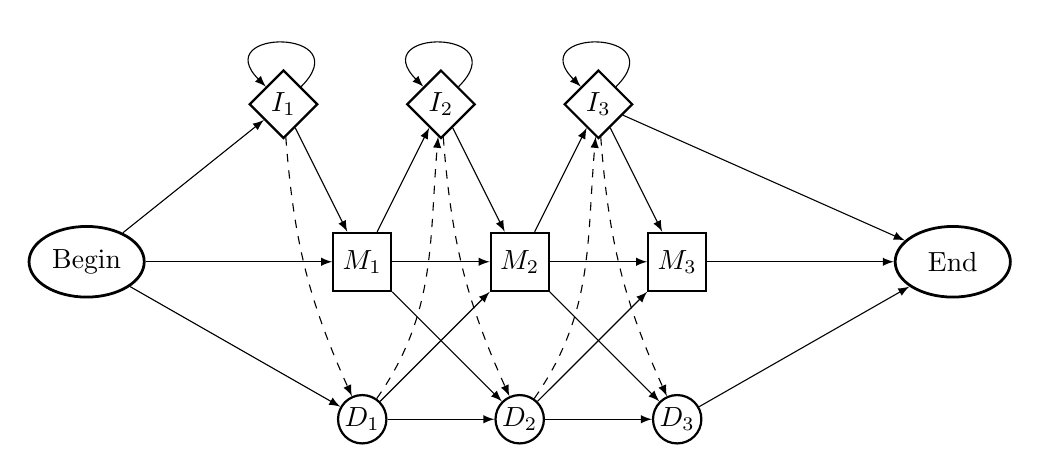
\begin{tikzpicture}[scale=1]  
		\tikzstyle{Match}=[rectangle,fit={(0,0) (0.5,0.5)},draw=Black,line width=0.8 pt, align=center]
		\tikzstyle{Deletion}=[circle,draw=Black,line width=0.8 pt, fit={(0,0) (0.2,0.2)}]
		\tikzstyle{Insertion}=[diamond,fit={(0,0) (0.2,0.2)},draw=Black,line width=0.8 pt]
		\tikzstyle{Border}=[ellipse,fit={(0,0) (0.8,0.4)},draw=Black,line width=1.0 pt]

 		\def\n {1}
 		\def\inSpace {2}
 		\def\Ishift {1}

		\foreach \i [count=\cnt] in {-\n,...,\n}
		{
			\node [Insertion] (I\i) at ({-\n + \inSpace * \i - \Ishift},2) {};
			\node [align=center] at (I\i.center) {$I_\cnt$};
			\node [Match] (M\i) at ({-\n + \inSpace * \i},0) {};
			\node [align=center] at (M\i.center) {$M_\cnt$};
			\node [Deletion] (D\i) at ({-\n + \inSpace * \i}, -2) {};
			\node [align=center] at (D\i.center) {$D_\cnt$};
			\pgfmathtruncatemacro{\ip}{\i + 1}
			\pgfmathtruncatemacro{\im}{\i - 1}
			
			\draw [dimen] (I\i) to[in=135,out=45, looseness=6] (I\i);
			\draw [dimen] (I\i) -- (M\i);
			\draw [dimen,dashed] (I\i) to[bend right=10] (D\i);
			
			\ifnum \i>-\n
				\draw [dimen] (M\im) -- (D\i);
				\draw [dimen] (M\im) -- (I\i);
				\draw [dimen] (M\im) -- (M\i);
				\draw [dimen] (D\im) -- (D\i);
				\draw [dimen] (D\im) -- (M\i);
				\draw [dimen,dashed] (D\im) to[out=55,in=-95] (I\i);
% 				\draw [dimen] (I\im) -- (I\i);
			\fi
		}
		
		\node [Border] (Begin) at ({-\n - \inSpace * \n - 3.5},0) {};
		\node [align=center] at ({-\n - \inSpace * \n - 3.5},0) {Begin};
		\node [Border] (End) at ({-\n + \inSpace * \n + 3.5},0) {};
		\node [align=center] at ({-\n + \inSpace * \n + 3.5},0) {End};
		\draw [dimen] (Begin) -- (D-\n);
        \draw [dimen] (Begin) -- (I-\n);
        \draw [dimen] (Begin) -- (M-\n);
        \draw [dimen] (D\n) -- (End);
        \draw [dimen] (I\n) -- (End);
        \draw [dimen] (M\n) -- (End);
		

  \end{tikzpicture}
	\caption{Simplified PfTools algorithm profile schema for a 3 sequence length profile. Simplifications arise from not showing all connections from Begin to nodes [$I_i$,$M_i$,$D_i$] as well as nodes [$I_i$,$M_i$,$D_i$] to End. It is worth noting the dashed that should not be used even though available. Indeed, mismatches should replace Insertion-Deletion or Deletion-Insertion paths thanks to extreme score loss.}
  \label{std prf}
\end{figure}

\begin{figure}[t]
  \centering
  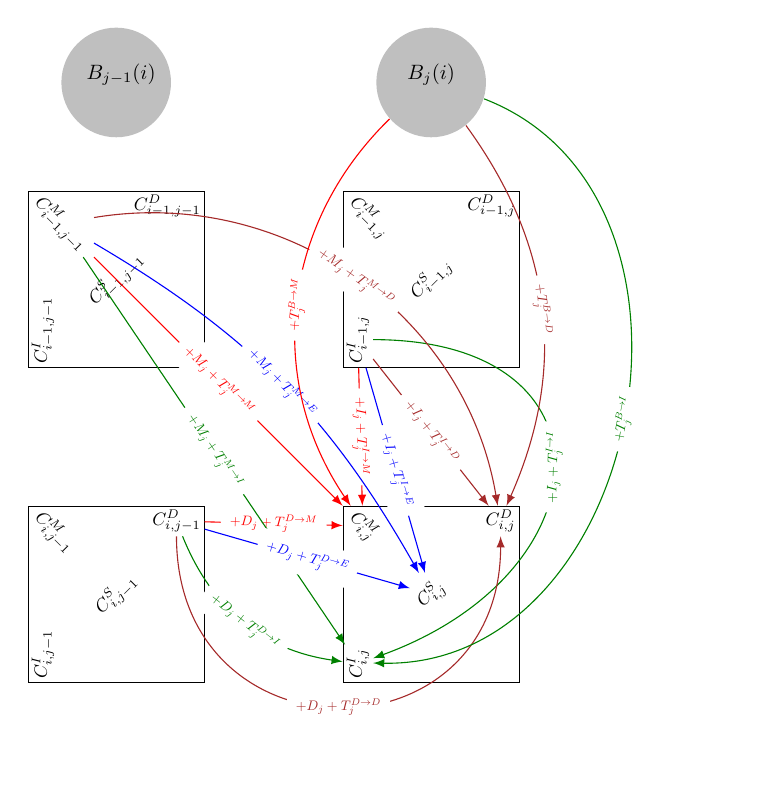
\begin{tikzpicture}[scale=1]   
%     \matrix (A) [column sep=5mm, row sep=3mm] {
%       \cell{$C^M_{i-1,j-1}$}{$C^I_{i-1,j-1}$}{$C^D_{i-1,j-1}$}{$C^S_{i-1,j-1}$}; &
%       \cell{$C^M_{i,j-1}$}{$C^I_{i,j-1}$}{$C^D_{i,j-1}$}{$C^S_{i,j-1}$}; \\
%       \cell{$C^M_{i-1,j}$}{$C^I_{i-1,j}$}{$C^D_{i-1,j}$}{$C^S_{i-1,j}$}; &
%       \cell{$C^M_{i,j}$}{$C^I_{i,j}$}{$C^D_{i,j}$}{$C^S_{i,j}$}; \\
%     };
    \node [myCell={$C^M_{i-1,j-1}$}{$C^I_{i-1,j-1}$}{$C^D_{i-1,j-1}$}{$C^S_{i-1,j-1}$}{A}] at (0,4) {};
    \node [myCell={$C^M_{i-1,j}$}{$C^I_{i-1,j}$}{$C^D_{i-1,j}$}{$C^S_{i-1,j}$}{B}] at (4,4) {};
    \node [myCell={$C^M_{i,j-1}$}{$C^I_{i,j-1}$}{$C^D_{i,j-1}$}{$C^S_{i,j-1}$}{C}] at (0,0) {};
    \node [myCell={$C^M_{i,j}$}{$C^I_{i,j}$}{$C^D_{i,j}$}{$C^S_{i,j}$}{D}] at (4,0) {};
    
    \node [circle, fill=lightgray, rounded corners=3pt, fit={(0,0) (.75,.75)}] at (0,6.5) {\scalebox{.75}{$B_{j-1}(i)$}};
    \node [circle, fill=lightgray, rounded corners=3pt, fit={(0,0) (.75,.75)}] (Bj) at (4,6.5) {\scalebox{.75}{$B_{j}(i)$}};
    
    \draw [red,dimen] (A Match) -- node {\scalebox{.5}{$+ M_j + T^{M\rightarrow M}_j$}} (D Match); 
    \draw [red,dimen] (B Insertion) -- node {\scalebox{.5}{$+ I_j + T^{I\rightarrow M}_j$}} (D Match);
    \draw [red,dimen] (C Deletion) -- node {\scalebox{.5}{$+ D_j + T^{D\rightarrow M}_j$}} (D Match);
    
    \draw [Green,dimen] (A Match) -- node {\scalebox{.5}{$+ M_j + T^{M\rightarrow I}_j$}} (D Insertion); 
    \draw [Green,dimen] (B Insertion) to[out=0,in=20,looseness=2] node {\scalebox{.5}{$+ I_j + T^{I\rightarrow I}_j$}} (D Insertion);
    \draw [Green,dimen] (C Deletion) to[bend right=30] node {\scalebox{.5}{$+ D_j + T^{D\rightarrow I}_j$}} (D Insertion);

    \draw [Brown,dimen] (A Match) to [bend left=45,looseness=1.] node {\scalebox{.5}{$+ M_j + T^{M\rightarrow D}_j$}} (D Deletion); 
    \draw [Brown,dimen] (B Insertion) -- node {\scalebox{.5}{$+ I_j + T^{I\rightarrow D}_j$}} (D Deletion);
    \draw [Brown,dimen] (C Deletion) to[bend right=90,looseness=1.8] node  {\scalebox{.5}{$+ D_j + T^{D\rightarrow D}_j$}} (D Deletion);

    \draw [blue,dimen] (A Match) to [bend left=15]  node {\scalebox{.5}{$+ M_j + T^{M\rightarrow E}_j$}} (D Extra); 
    \draw [blue,dimen] (B Insertion) --  node {\scalebox{.5}{$+ I_j + T^{I\rightarrow E}_j$}} (D Extra);
    \draw [blue,dimen] (C Deletion) -- node {\scalebox{.5}{$+ D_j + T^{D\rightarrow E}_j$}} (D Extra);

    \draw [red, dimen] (Bj) to[bend right=40] node {\scalebox{.5}{$+T^{B\rightarrow M}_j$}} (D Match);
    \draw [Brown, dimen] (Bj) to[bend right=-30] node {\scalebox{.5}{$+T^{B\rightarrow D}_j$}} (D Deletion);
    \draw [Green, dimen] (Bj) to[bend left=80, looseness=1.2] node {\scalebox{.5}{$+T^{B\rightarrow I}_j$}} (D Insertion);
    
  \end{tikzpicture}
  \caption{Standard PfTools algorithm schema}
  \label{std}
\end{figure}
\begin{figure}[p]
  \centering
  \begin{tikzpicture}[scale=2]   
%     \matrix (A) [column sep=5mm, row sep=3mm] {
%       \cell{$C^M_{i-1,j-1}$}{$C^I_{i-1,j-1}$}{$C^D_{i-1,j-1}$}{$C^S_{i-1,j-1}$}; &
%       \cell{$C^M_{i,j-1}$}{$C^I_{i,j-1}$}{$C^D_{i,j-1}$}{$C^S_{i,j-1}$}; \\
%       \cell{$C^M_{i-1,j}$}{$C^I_{i-1,j}$}{$C^D_{i-1,j}$}{$C^S_{i-1,j}$}; &
%       \cell{$C^M_{i,j}$}{$C^I_{i,j}$}{$C^D_{i,j}$}{$C^S_{i,j}$}; \\
%     };
    \node [myCell={$C^M_{i-1,j-1}$}{$C^I_{i-1,j-1}$}{$C^D_{i-1,j-1}$}{$C^S_{i-1,j-1}$}{A}] at (0,4) {};
    \node [myCell={$C^M_{i-1,j}$}{$C^I_{i-1,j}$}{$C^D_{i-1,j}$}{$C^S_{i-1,j}$}{B}] at (4,4) {};
    \node [myCell={$C^M_{i,j-1}$}{$C^I_{i,j-1}$}{$C^D_{i,j-1}$}{$C^S_{i,j-1}$}{C}] at (0,0) {};
    \node [myCell={$C^M_{i,j}$}{$C^I_{i,j}$}{$C^D_{i,j}$}{$C^S_{i,j}$}{D}] at (4,0) {};
    
    \draw [red,dimen] (A Match) -- node {\scalebox{.5}{$+ M_j + T^{M\rightarrow M}_j$}} (D Match); 
    \draw [red,dimen] (B Insertion) -- node {\scalebox{.5}{$+ I_j + T^{I\rightarrow M}_j$}} (D Match);
    \draw [red,dimen] (C Deletion) -- node {\scalebox{.5}{$+ D_j + T^{D\rightarrow M}_j$}} (D Match);
    
    \draw [Green,dimen] (A Match) -- node {\scalebox{.5}{$+ M_j + T^{M\rightarrow I}_j$}} (D Insertion); 
    \draw [Green,dimen] (B Insertion) to[out=0,in=20,looseness=1] node {\scalebox{.5}{$+ I_j + T^{I\rightarrow I}_j$}} (D Insertion);

    \draw [Blue,dimen] (A Match) to [bend left=45,looseness=1.] node {\scalebox{.5}{$+ M_j + T^{M\rightarrow D}_j$}} (D Deletion); 
    \draw [Blue,dimen] (C Deletion) to[bend right=90,looseness=1.8] node  {\scalebox{.5}{$+ D_j + T^{D\rightarrow D}_j$}} (D Deletion);
    
  \end{tikzpicture}
  \caption{Standard PfTools algorithm schema}
  \label{std_app}
\end{figure}

Let us define the indexing function $f(s): \A \mapsto [1,N_\alpha]$ which translate the character $s$ of the alphabet $\A$ 
into its corresponding index within the score tables $M$, $I$.   
The recurrence relations for $C^\alpha_{i,j}$, $\alpha \in \{M,I,D,S\}$ pictured in figure \ref{std} are as follow:
\begin{equation} \label{std1} \arraycolsep=1.4pt\def\arraystretch{1.7}
	C_{i,j}^{M} = \left \{
		\begin{array}{c l l}
		  F^{M}_0 &,& i = 0,\, j = 0\\
		  
		  \max & \left \{
		  \begin{array} {ccccc}
		  C_{0,j-1}^{D}   &+& D_{j} &+& T^{D \rightarrow M}_j \\
		  F^{M}_j \\
		  \end{array} \right. , & i = 0,\, j \in [1,N_p]\\
		  
		  \max & \left \{
		  \begin{array} {ccccc}
		  C_{i-1,0}^{I}   &+& I_{j, f(s_i)} &+& T^{I \rightarrow M}_0 \\
		  T^{B \rightarrow M}_0 \\
		  \end{array} \right. , & i \in [1,N_s-1],\, j = 0 \\
		
		  \max & \left \{
		  \begin{array} {ccccc}
		  C_{i-1,j-1}^{M} &+& M_{j, f(s_i)} &+& T^{M \rightarrow M}_j \\
		  C_{i-1,j}^{I}   &+& I_{j, f(s_i)} &+& T^{I \rightarrow M}_j \\
		  C_{i,j-1}^{D}   &+& D_{j} &+& T^{D \rightarrow M}_j \\
		  T^{B \rightarrow M}_j \\
		  \end{array} \right. , & i \in [1,N_s-1],\, j \in [1,N_p]\\
		\end{array}
		\right.
\end{equation}

\begin{equation} \label{std2} \arraycolsep=1.4pt\def\arraystretch{1.7}
  C_{i,j}^{I} = \left \{
		\begin{array}{c l l}
		  F^{I}_0 &,& i = 0,\, j = 0\\
		  
		  \max & \left \{
		  \begin{array} {ccccc}
		  C_{0,j-1}^{D}   &+& D_{j} &+& T^{D \rightarrow I}_j \\
		  F^{I}_j \\
		  \end{array} \right. , & i = 0,\, j \in [1,N_p]\\
		  
		  \max & \left \{
		  \begin{array} {ccccc}
		  C_{i-1,0}^{I}   &+& I_{f(s_i),0} &+& T^{I \rightarrow I}_0 \\
		  T^{B \rightarrow I}_0 \\
		  \end{array} \right. , & i \in [1,N_s-1],\, j = 0 \\
		
		  \max & \left \{
		  \begin{array} {ccccc}
		  C_{i-1,j-1}^{M} &+& M_{j, f(s_i)} &+& T^{M \rightarrow I}_j \\
		  C_{i-1,j}^{I}   &+& I_{j, f(s_i)} &+& T^{I \rightarrow I}_j \\
		  C_{i,j-1}^{D}   &+& D_{j} &+& T^{D \rightarrow I}_j \\
		  T^{B \rightarrow I}_j \\
		  \end{array} \right. , & i \in [1,N_s-1],\, j \in [1,N_p]\\
		\end{array}
		\right.
\end{equation}

\begin{equation} \label{std3} \arraycolsep=1.4pt\def\arraystretch{1.7}
  C_{i,j}^{D} = \left \{
		\begin{array}{c l l}
		  F^{D}_0 &,& i = 0,\, j = 0\\
		  
		  \max & \left \{
		  \begin{array} {ccccc}
		  C_{i,j-1}^{D}   &+& D_{j} &+& T^{D \rightarrow D}_j \\
		  F^{M}_j \\
		  \end{array} \right. , & i = 0,\, j \in [1,N_p]\\
		  
		  \max & \left \{
		  \begin{array} {ccccc}
		  C_{i-1,0}^{I}   &+& I_{j, f(s_i)} &+& T^{I \rightarrow D}_j \\
		  T^{B \rightarrow M}_0 \\
		  \end{array} \right. , & i \in [1,N_s-1],\, j = 0 \\
		
		  \max & \left \{
		  \begin{array} {ccccc}
		  C_{i-1,j-1}^{M} &+& M_{j, f(s_i)} &+& T^{M \rightarrow D}_j \\
		  C_{i-1,j}^{I}   &+& I_{j, f(s_i)} &+& T^{I \rightarrow D}_j \\
		  C_{i,j-1}^{D}   &+& D_{j} &+& T^{D \rightarrow D}_j \\
		  T^{B \rightarrow D}_j \\
		  \end{array} \right. , & i \in [1,N_s-1],\, j \in [1,N_p]\\
		\end{array}
		\right.
\end{equation}

\begin{equation} \label{std4} \arraycolsep=1.4pt\def\arraystretch{1.7}
  C_{i,j}^{S} = \left \{
		\begin{array}{c l l}
		  		
		  \max & \left \{
		  \begin{array} {ccccc}
		  C_{i-1,j-1}^{M} &+& M_{j, f(s_i)} &+& T^{M \rightarrow E}_j \\
		  C_{i-1,j}^{I}   &+& I_{j, f(s_i)} &+& T^{I \rightarrow E}_j \\
		  C_{i,j-1}^{D}   &+& D_{j} &+& T^{D \rightarrow E}_j \\
		  \end{array} \right. , & i \in [1,N_s-1],\, j \in [1,N_p]\\
		  
		  \max & \left \{
		  \begin{array} {ccccc}
		  C_{i-1,j-1}^{M} &+& M_{j, f(s_i)} &+& L^{M}_j \\
		  C_{i-1,j}^{I}   &+& I_{j, f(s_i)} &+& L^{I}_j \\
		  C_{i,j-1}^{D}   &+& D_{j} &+& L^{D}_j \\
		  \end{array} \right. , & i = N_s,\, j \in [1,N_p]\\
		  
		  \mathrm{useless} &,& i = 0 \,\,\mathrm{or}\,\, j = 0
		  
		\end{array}
		\right.
\end{equation}

Running PfSearch, either version 2 or 3, first computes the cell matrix $C^\alpha_{i,j}$, $\alpha \in \{M,I,D,S\}$, then 
analyzes the latter looking for the best match i.e. the highest score $C^S_{k,l}$ where the range of $l$ is in agreement with 
the type of alignment sought. For a \emph{global} alignment, one enforces the match to end on the last profile position, hence $l=N_p$. On the other hand, a \emph{local} alignment
allows $l \in [0,N_p]$. It is worth mentionning that any type of alignment is also subject to the profile declaration and therefore
it may well happen that the backward tracing encounters an entry point before reaching the profile's length. As an example, one
can try to elucidate the path given in figure \ref{Testexample}.

\section{Repeat Decoder}

The Repeat detecter algorithm is a bit more complex than the standard PfTools one as it incorporates feedback loop to accomodate potential replication of the profile.
\begin{figure}[t]
  \centering
  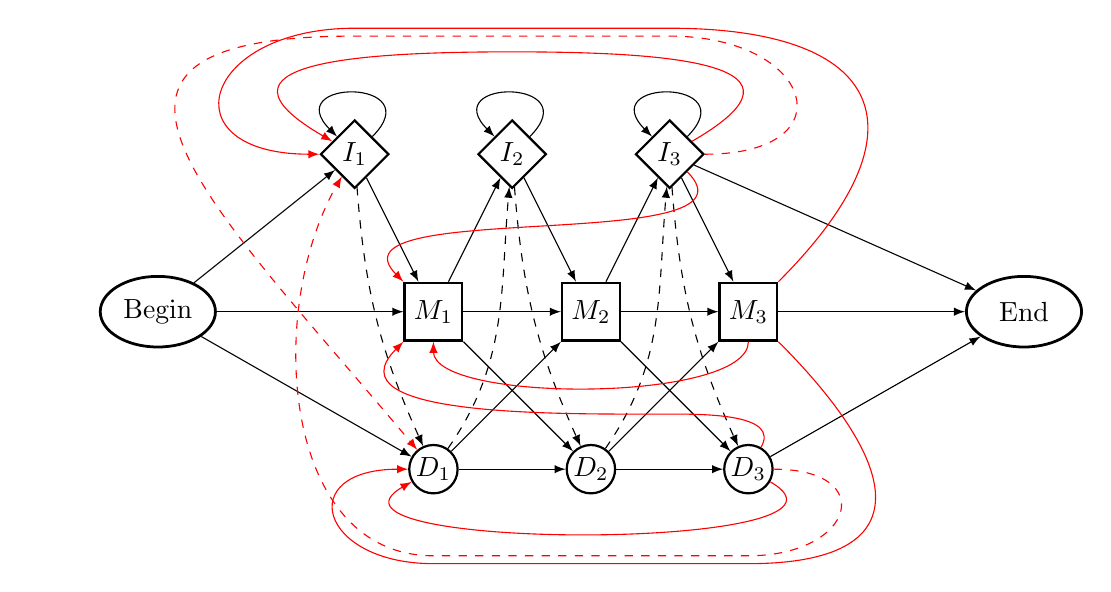
\begin{tikzpicture}[scale=1]  
		\tikzstyle{Match}=[rectangle,fit={(0,0) (0.5,0.5)},draw=Black,line width=0.8 pt, align=center]
		\tikzstyle{Deletion}=[circle,draw=Black,line width=0.8 pt, fit={(0,0) (0.2,0.2)}]
		\tikzstyle{Insertion}=[diamond,fit={(0,0) (0.2,0.2)},draw=Black,line width=0.8 pt]
		\tikzstyle{Border}=[ellipse,fit={(0,0) (0.8,0.4)},draw=Black,line width=1.0 pt]

 		\def\n {1}
 		\def\inSpace {2}
 		\def\Ishift {1}

		\foreach \i [count=\cnt] in {-\n,...,\n}
		{
			\node [Insertion] (I\i) at ({-\n + \inSpace * \i - \Ishift},2) {};
			\node [align=center] at (I\i.center) {$I_\cnt$};
			\node [Match] (M\i) at ({-\n + \inSpace * \i},0) {};
			\node [align=center] at (M\i.center) {$M_\cnt$};
			\node [Deletion] (D\i) at ({-\n + \inSpace * \i}, -2) {};
			\node [align=center] at (D\i.center) {$D_\cnt$};
			\pgfmathtruncatemacro{\ip}{\i + 1}
			\pgfmathtruncatemacro{\im}{\i - 1}
			
			\draw [dimen] (I\i) to[in=135,out=45, looseness=6] (I\i);
			\draw [dimen] (I\i) -- (M\i);
			\draw [dimen,dashed] (I\i) to[bend right=10] (D\i);
			
			\ifnum \i>-\n
				\draw [dimen] (M\im) -- (D\i);
				\draw [dimen] (M\im) -- (I\i);
				\draw [dimen] (M\im) -- (M\i);
				\draw [dimen] (D\im) -- (D\i);
				\draw [dimen] (D\im) -- (M\i);
				\draw [dimen,dashed] (D\im) to[out=55,in=-95] (I\i);
% 				\draw [dimen] (I\im) -- (I\i);
			\fi
		}
		
		\node [Border] (Begin) at ({-\n - \inSpace * \n - 3.5},0) {};
		\node [align=center] at ({-\n - \inSpace * \n - 3.5},0) {Begin};
		\node [Border] (End) at ({-\n + \inSpace * \n + 3.5},0) {};
		\node [align=center] at ({-\n + \inSpace * \n + 3.5},0) {End};
		\draw [dimen] (Begin) -- (D-\n);
        \draw [dimen] (Begin) -- (I-\n);
        \draw [dimen] (Begin) -- (M-\n);
        \draw [dimen] (D\n) -- (End);
        \draw [dimen] (I\n) -- (End);
        \draw [dimen] (M\n) -- (End);
        
        \pgfmathtruncatemacro{\first}{-\n}
        \pgfmathtruncatemacro{\last}{\n}
        \draw [dimen,red] (I\last) to[out=30, in=0, looseness=2] ({-\n + \inSpace * 0 - \Ishift},3.3) to[out=180,in=150,looseness=2] (I\first);
        \draw [dimen,red] (I\last) to[out=-45, in=135] (M\first);
        
        \draw [dimen,red] (D\last) to[in=-150, out=-30] (D\first);
        \draw [dimen,red] (D\last) to[in=0, out=60] (0,-1.3) to[out=180,in=-135] (M\first);
        
        \draw [dimen,red] (M\last) to[in=-90, out=-90, looseness=.5]  (M\first);
        \draw [dimen,red] (M\last) to[in=0, out=45, looseness=2] ({-\n +\n*\inSpace - \Ishift},3.6) -- ({-\n -\n*\inSpace - \Ishift},3.6) to[out=180,in=180,looseness=3] (I\first);
        \draw [dimen,red] (M\last) to[in=0, out=-45, looseness=2] (-\n + \n*\inSpace,-3.2) -- ({-\n - \n*\inSpace },-3.2) to[out=180,in=180,looseness=3] (D\first);
		
		\draw [dimen,dashed,red] (I\last) to[out=0,in=0, looseness=3] ({-\n +\n*\inSpace - \Ishift},3.5) -- ({-\n -\n*\inSpace - \Ishift},3.5) to[out=180,in=130,looseness=2](D\first);
		\draw [dimen,dashed,red] (D\last) to[in=0, out=0, looseness=3] (-\n + \n*\inSpace,-3.1) -- ({-\n - \n*\inSpace },-3.1) to[out=180,in=-120] (I\first);
		

  \end{tikzpicture}
	\caption{Simplified PfTools algorithm profile schema for a 3 sequence length profile. Simplifications arise from not showing all connections from Begin to nodes [$I_i$,$M_i$,$D_i$] as well as nodes [$I_i$,$M_i$,$D_i$] to End. It is worth noting the dashed lines that should not be used even though available. Indeed, mismatches should replace Insertion-Deletion or Deletion-Insertion paths thanks to extreme score loss.}
  \label{std prf}
\end{figure}


\end{document}
